\documentclass{article}
\usepackage[T1]{fontenc}
\usepackage[utf8]{inputenc}

% Language setting
% Replace `english' with e.g. `spanish' to change the document language
% Idioma sin shorthands conflictivos para bibpunct
\usepackage[spanish,es-noshorthands]{babel} 
\spanishdecimal.
% Set page size and margins
% Replace `letterpaper' with`a4paper' for UK/EU standard size
\usepackage[letterpaper,top=2cm,bottom=2cm,left=3cm,right=3cm,marginparwidth=1.75cm]{geometry}

% Useful packages
\usepackage{booktabs}
\usepackage{amsmath}
\usepackage{graphicx}
\usepackage{float}
\usepackage{times}
\usepackage{natbib}
\usepackage[colorlinks=true, allcolors=blue]{hyperref}
\usepackage{graphics}
%\usepackage[sf,bf,tiny,center,compact]{titlesec}
%Cambiar quizá por sub Caption
%\usepackage{subfigure}
\usepackage{tabularx}
\usepackage{amssymb}
\usepackage{mathrsfs}
\usepackage{hyphenat}
\usepackage{tikz}
\usepackage{blox}
\hyphenation{co-mer-cial rea-li-zan si-guien-te si-mu-la-ción ke-lly con-si-de-ra-da}
\AtBeginDocument{\bibpunct{(}{)}{;}{a}{,}{,}}

%Variables Comúnes:
\newcommand{\EstudianteA}{Breña Torres Axel Ivan}
\newcommand{\EstudianteB}{Davalos Salina Diego Alberyo}
\newcommand{\EstudianteC}{Jiménes Herrera Daniela}
\newcommand{\EstudianteD}{Paredes Lara Kevin}
\newcommand{\EstudianteE}{Peña Pérez Calli Yereki}
\newcommand{\EstudianteF}{Trejo Mendoza Aaron Emmanuel}
\newcommand{\NumeroPractica}{01}
\newcommand{\TituloPractica}{Respuesta en frecuencia de filtros RC pasa bajas y pasa altas de primer orden}
\newcommand{\FechaCompromiso}{25 de septiembre de 2026}
\newcommand{\FechaEntrega}{\today}

\begin{document}

%portada
\begin{titlepage}
\centering
	\begin{figure}
  \begin{minipage}{1\linewidth}
     \centering\centering%\rule{2cm}{2cm}
    % \caption{Primera figura}
    
\includegraphics[width=0.3\textwidth]{img/logos_fi_uaq.png}
     
  \end{minipage}
\end{figure}
{\scshape\LARGE Universidad Autónoma de Querétaro \par}
	\vspace{0.5cm}
	{\scshape\Large Facultad de Ingeniería \par}
	\vspace{0.5cm}
	{\scshape\Large Ingeniería en Automatización \par}
	\vspace{0.5cm}	
	{\Large\bfseries Control II\par}
	\vspace{0.8cm}
	{\Large\bfseries \TituloPractica \\ \par}	
	\vspace{0.8cm}
	{\Large\itshape Práctica \NumeroPractica\par}
	\vspace{0.8cm}
	Profesor: \par
	Dr. Roberto Valentín Carrillo Serrano \par
	\vspace{0.5cm}
	Equipo 1\par \vspace{0.2cm}
	Integrantes:\vspace{0.4cm}
\par	
	\EstudianteA \hfill \rule{70mm}{0.1mm}
\vspace{0.4cm}
\par    
    \EstudianteB \hfill \rule{70mm}{0.1mm}
\vspace{0.4cm}
\par
    \EstudianteC \hfill \rule{70mm}{0.1mm}
\vspace{0.4cm}
\par
    \EstudianteD \hfill \rule{70mm}{0.1mm}
\vspace{0.4cm}
\par
    \EstudianteE \hfill \rule{70mm}{0.1mm}
\vspace{0.4cm}
\par
    \EstudianteF \hfill \rule{70mm}{0.1mm}

\par
	
		
	\vfill

% Bottom of the page
	{\large Fecha compromiso: \FechaCompromiso\par
    Fecha en que se entregó: \FechaEntrega}.
\end{titlepage}

%\frontmatter	%fija la numeración romana
\thispagestyle{empty}%no imprimir número de página en índice
\tableofcontents
\listoffigures
\listoftables
%\printindex
\newpage
%\setcounter{page}{1}
%\mainmatter 	%fija la numeración arábiga



\section{Objetivo}
Construir un filtro RC pasa bajas de primer orden y un filtro RC pasa altas de primer orden para ver su respuesta en frecuencia en el osciloscopio, graficando el comportamiento de la magnitud y de la fase ante una señal sinusoidal de entrada con una amplitud constante y diferentes frecuencias

\section{Marco Teórico}
Si a un proceso $G(s)$ cualquiera le aplicamos un a la entrada una señal en forma de seno o coseno, la manera en que cambian la amplitud y la fase de la señal de salida depende de cómo son y en dónde están ubicados los polos y ceros de la función de transferencia de nuestra planta (\cite{notasclase}). 

\begin{figure}[H]
    \centering
    
\includegraphics[width=0.5\linewidth]{BaseReporte2026-1/entrada_salida.png}
    \caption{Relación entre la amplitud y fase de las señales de entrada y salida}
    \label{fig:vi_vo}
\end{figure}

La idea básica de la respuesta en frecuencia es que si se le aplica una entrada sinusoidal cualquiera, $v_i$, el cual está representado por:

\begin{equation}
	v_i = A\sin(wt)
	\label{eq:entrada_vi}
\end{equation}

Donde $w$ es la frecuencia en $[\frac{rad}{s}]$.
En la salida del sistema obtendremos una señal sinusoidal la cual dependiendo de la función de transferencia, saldrá con otra amplitud y una fase distinta con relación con la señal aplicada a la entrada, la cual podemos representar como: 

\begin{equation}
    v_o=B\sin(wt+\phi )
    \label{eq:salida_vo}
\end{equation}

Donde $\phi$ es el ángulo de fase o simplemente la fase y se obtiene a partir de la siguiente ecuación:

\begin{equation}
    \phi = \frac{360\,[^\circ]}{T}t_\phi
    \label{eq:phi}
\end{equation}

\subsection{Filtro RC pasa bajas}
En la Figura~\ref{fig:RC_pasabajas} se presenta el diagrama de un experimento de un circuito RC (configuración pasa bajas) de corriente alterna.

\begin{figure}[H]
\centering
    
\includegraphics[width=0.4\linewidth]{BaseReporte2026-1/Circuito_RC.png}
    \caption{Diagrama del circuito RC.}
    \label{fig:RC_pasabajas}
\end{figure}

Donde sus voltajes de entrada y de salida están dados por:

\begin{equation}
    v_i = Ri+\frac{1}{c}\int_{0}^{t}i(\tau)d\tau, \quad v_o = \frac{1}{c}\int_{0}^{t}i(\tau)d\tau
    \label{eq:voltajes_entrada_salida}
\end{equation}

Pasando a Laplace tenemos:

\begin{equation}
    V_i(s) = RI(s)+\frac{1}{C}*\frac{1}{s}I(s), \quad V_o(s) = \frac{1}{Cs}I(s)
    \label{eq:voltajes_entrada_salida_laplace}
\end{equation}

Finalmente, la función de transferencia en el dominio de Laplace se representa como: 

\begin{equation}
    G(s) = \frac{V_o(s)}{V_i(s)} = \frac{1}{RCs+1} = \frac{a}{s+a}
    \label{eq:Fun_transf_pasabajas}
\end{equation}

Donde para la forma polo-cero: 

\begin{equation}
    a = \frac{1}{RC}
    \label{eq:polo-cero-pb}
\end{equation}

Combinando estas expresiones, obtenemos: 

\begin{equation}
    V_o(s) = \frac{a}{s+a}V_i(s), \quad a = \frac{1}{RC}
\end{equation}

Realizamos el cambio de variable $s = jw$, obteniendo la siguiente ecuación:

\begin{equation}
    G(jw)  = \frac{a}{a+jw} 
\end{equation}

Multiplicando por el factor $\frac{a-jw}{a-jw}$ obtenemos: 

\begin{equation}
    G(jw) = \frac{a}{a+jw}\left[\frac{a-jw}{a-jw}\right] = \frac{a(a-jw)}{a^2-(jw)^2} = \frac{a(a-jw)}{a^2+w^2}
\end{equation}

Para la magnitud $|G(jw)|$ recordemos que toda función de transferencia se define como el cociente de la salida entre la entrada (\cite{notasclase}): 

\begin{equation}
    |G(jw)| = \left|\frac{a(a-jw)}{a^2+w^2}\right| = \frac{|a(a-jw)|}{a^2+w^2} = \frac{a\sqrt{a^2+w^2}}{\sqrt{a^2+w^2}\sqrt{a^2+w^2}} = \frac{a}{\sqrt{a^2+w^2}} = \frac{A}{B}
    \label{eq:Magnitud_pb}
\end{equation}

Para el caso de la fase $\angle G(jw) = \phi$ recordemos que los ceros aportan fase positiva mientras que los polos aportan fase negativa, además de la identidad $-\arctan(\alpha) = \arctan(-\alpha)$ (\cite{notasclase}):

\begin{equation}
    \phi = \angle G(jw) = \angle \left(\frac{a}{a+jw}\right) = 0-\angle (a+jw) = -\arctan\left(\frac{w}{a}\right)
    \label{eq:fase_pb}
\end{equation}

\subsection{Filtro RC pasa altas}
Para el circuito RC (configurado en pasa altas), la resistencia y el capacitor cambian de lugar, por ende, sus voltajes de entrada y salida están dados por: 

\begin{equation}
    v_i = \frac{1}{c}\int_{0}^{t}i(\tau)d\tau+Ri, \quad v_o = Ri
\end{equation}

Pasando a Laplace tenemos: 

\begin{equation}
    V_i (s) = \frac{1}{Cs}I(s) + RI(s), \quad V_o(s) = RI(s)
\end{equation}

La función de transferencia en el dominio de Laplace se representa como: 

\begin{equation}
    G(s) = \frac{V_o (s)}{V_i(s)} = \frac{s}{s+\frac{1}{RC}} = \frac{s}{s+a}, \quad a=\frac{1}{RC}
\end{equation}

Realizamos el cambio de variable $s = jw$, obteniendo la siguiente ecuación:

\begin{equation}
    G(jw) = \frac{jw}{jw + a}
\end{equation}

Multiplicando por el factor $\frac{a-jw}{a-jw}$, obtenemos: 

\begin{equation}
    G(jw) = \frac{jw}{a + jw}\left[\frac{a-jw}{a-jw}\right] = \frac{jw(a-jw)}{a^2-(jw)^2} = \frac{jwa+w^2}{a^2+w^2}
\end{equation}

Para la magnitud $|G(jw)|$ recordemos que toda función de transferencia se define como el cociente de la salida entre la entrada (\cite{notasclase}): 

\begin{equation}
    |G(jw)| = \left|\frac{jwa+w^2}{a^2+w^2}\right| = \frac{|w(ja+w)|}{a^2+w^2} = \frac{w\sqrt{a^2+w^2}}{\sqrt{a^2+w^2}\sqrt{a^2+w^2}} = \frac{w}{\sqrt{a^2+w^2}} 
    \label{eq:Magnitud_pa}
\end{equation}


Para el caso de la fase $\angle G(jw) = \phi$ recordemos que los ceros aportan fase positiva mientras que los polos aportan fase negativa, además de la identidad $-\arctan(\alpha) = \arctan(-\alpha)$ (\cite{notasclase}):

\begin{equation}
    \begin{aligned}
         \phi = \angle G(jw) = \angle \left(\frac{jw}{a+jw}\right) = \angle jw-\angle (a+jw) \\ = \arctan\left(\frac{w}{0}\right) -\arctan\left(\frac{w}{a}\right)= 90\,[^\circ] - \arctan \left(\frac{w}{a}\right)
        \label{eq:fase_pa}
    \end{aligned}
\end{equation}

\subsection{Filtro RC pasa altas}
En la Figura~\ref{fig:RC_pasaaltas} se presenta el diagrama de un experimento de un circuito RC (configuración pasa altas) de corriente alterna.


%\begin{figure}[H]
%\centering
 %   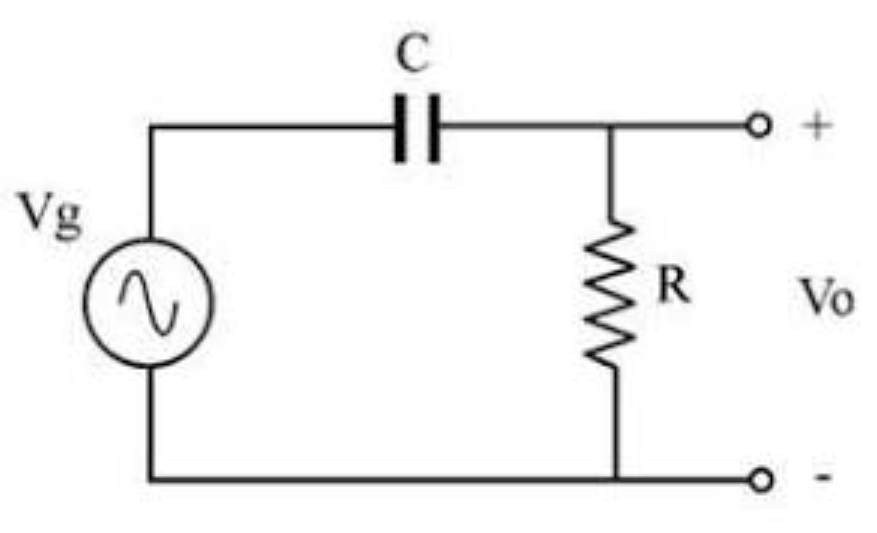
\includegraphics[width=0.4\linewidth]{img/Circuito_RC_altas.png}
  %  \caption{Diagrama del circuito RC.}
   % \label{fig:RC_pasaaltas}
%\end{figure}

Para el circuito RC (configurado en pasa altas), la resistencia y el capacitor cambian de lugar, por ende, sus voltajes de entrada y salida están dados por: 

\begin{equation}
    v_i = \frac{1}{c}\int_{0}^{t}i(\tau)d\tau+Ri, \quad v_o = Ri
\end{equation}

Pasando a Laplace tenemos: 

\begin{equation}
    V_i (s) = \frac{1}{Cs}I(s) + RI(s), \quad V_o(s) = RI(s)
\end{equation}

La función de transferencia en el dominio de Laplace se representa como: 

\begin{equation}
    G(s) = \frac{V_o (s)}{V_i(s)} = \frac{s}{s+\frac{1}{RC}} = \frac{s}{s+a}, \quad a=\frac{1}{RC}
\end{equation}

Realizamos el cambio de variable $s = jw$, obteniendo la siguiente ecuación:

\begin{equation}
    G(jw) = \frac{jw}{jw + a}
\end{equation}

Multiplicando por el factor $\frac{a-jw}{a-jw}$, obtenemos: 

\begin{equation}
    G(jw) = \frac{jw}{a + jw}\left[\frac{a-jw}{a-jw}\right] = \frac{jw(a-jw)}{a^2-(jw)^2} = \frac{jwa+w^2}{a^2+w^2}
\end{equation}

Para la magnitud $|G(jw)|$ recordemos que toda función de transferencia se define como el cociente de la salida entre la entrada (\cite{notasclase}): 

\begin{equation}
    |G(jw)| = \left|\frac{jwa+w^2}{a^2+w^2}\right| = \frac{|w(ja+w)|}{a^2+w^2} = \frac{w\sqrt{a^2+w^2}}{\sqrt{a^2+w^2}\sqrt{a^2+w^2}} = \frac{w}{\sqrt{a^2+w^2}} 
    \label{eq:Magnitud_pa}
\end{equation}


Para el caso de la fase $\angle G(jw) = \phi$ recordemos que los ceros aportan fase positiva mientras que los polos aportan fase negativa, además de la identidad $-\arctan(\alpha) = \arctan(-\alpha)$ (\cite{notasclase}):

\begin{equation}
    \begin{aligned}
         \phi = \angle G(jw) = \angle \left(\frac{jw}{a+jw}\right) = \angle jw-\angle (a+jw) \\ = \arctan\left(\frac{w}{0}\right) -\arctan\left(\frac{w}{a}\right)= 90\,[^\circ] - \arctan \left(\frac{w}{a}\right)
        \label{eq:fase_pa}
    \end{aligned}
\end{equation}



\section{Materiales y Métodos}
Para la realización de la práctica se utilizaron los siguientes materiales:
\begin{itemize}

	\item Resistencia de $67\ [k\Omega]$.
	\item Capacitor de $6.7\ [\mu F]$.
	\item Soldura de estaño.
	\item Estación de soldadura.
	\item Generador de funciones.
	\item Osciloscopio digital.
	
\end{itemize}

Igualmente, se utilizó el software de hoja de cálculo \textit{Excel} para graficar los resultados 
medidos con el osciloscopio y los resultados teoricos obtenidos a partir de las formulas especificadas 
en el Marco Teórico.

\subsection{Creación del Circuito}
Se construyón el circuito RC pasa bajas de primer orden siguiendo el diagrama de la 
Figura~\ref{fig:RC_pasabajas}, soldando las terminales de la resistencia y del capacitor
entre sí, con el propósito de reducir la resistencia de contacto y evitar que se generen
errores en la medición de la señal de salida.

\subsection{Generación de la señal de entrada}
Se generó una señal sinusoidal de entrada con una amplitud constante de $1\ [V]$
y diferentes frecuencias propuestas en $[\frac{rad}{s}]$, las cuales fueron calculadas
también en $[Hz]$ para poder ser introducidas en el generador de funciones. La sonda
positiva del osciloscopio se conectó a la salida del generador de funciones y la sonda
negativa a tierra, para poder medir la señal de entrada.

\subsection{Medición de la señal de salida}
Con la ayuda de los cursores del osciloscopio, se midió la amplitud de la señal de salida
en $[V]$ y el tiempo de retardo en $[ms]$ con respecto a la señal de entrada, para poder
calcular así el desfase en grados. La señal de salida se midió conectando la sonda positiva
del osciloscopio a la salida del circuito y la sonda negativa a tierra.

\subsection{Cálculo de la magnitud y del desfase}
Una vez obtenidos los valores de la amplitud de la señal de salida y del tiempo de retardo, 
se calculó la ganancia en $[dB]$ y el desfase en $[rad]$ con las siguientes ecuaciones:
\begin{equation}
    G = \frac{V_o}{V_i}
    \label{eq:ganancia}
\end{equation}

\begin{equation}
    G_{\mathrm{dB}} = 20\log_{10}\left(\frac{V_o}{V_i}\right)
    \label{eq:ganancia_db}
\end{equation}

\begin{equation}
    \phi = \omega t_{\phi}
    = 2\pi f t_{\phi}
    = \frac{2\pi t_{\phi}}{T}
    \quad [\,{^\circ}]
    \label{eq:desfase_rad}
\end{equation}

Todos estos cálculos se realizaron en la hoja de cálculo \textit{Excel} 
para poder, posteriorente, graficar los resultados obtenidos.


\section{Resultados y Discusión}
A continuación se presentan los resultados obtenidos en la práctica, 
tanto experimentales como teóricos de ambos filtros, así como la 
discusion individual de cada integrante del equipo y la discusión 
colectiva.

\subsection{Resultado Experimentales}
Los siguientes datos fueron registrados con ayuda del osciloscopio 
digital, adquiridos por medio de los cursores del mismo.

\subsubsection{Filtro Pasa Bajas}
\begin{table}[H]
\centering
\caption{Respuesta en frecuencia experimental del Filtro Pasa Bajas}
\label{tab:filtro_pasabajas}
\begin{tabular}{ccccccc}
	\toprule
	
$\omega$ & $f$ & $V_{i}$ & $V_{o}$ & Ganancia & $\Delta t$ & $\phi$ \\
$[\frac{{rad}}{{s}}]$ & {$[Hz]$} & $[V]$ & $[V]$ & $[dB]$ & $[ms]$ & $[^\circ]$ \\
\midrule
10    & 1.592    & 1.00 & 1.00 &   0.0000 & 0.000 &   0.0000 \\
20    & 3.185    & 1.00 & 1.00 &   0.0000 & 0.000 &   0.0000 \\
30    & 4.777    & 1.00 & 1.00 &   0.0000 & 0.200 &  -0.3439 \\
40    & 6.369    & 1.00 & 1.00 &   0.0000 & 0.480 &  -1.1006 \\
50    & 7.962    & 1.00 & 1.00 &   0.0000 & 0.670 &  -1.9204 \\
60    & 9.554    & 1.00 & 1.00 &   0.0000 & 1.000 &  -3.4395 \\
70    & 11.146   & 1.00 & 0.99 &  -0.0873 & 1.000 &  -4.0127 \\
80    & 12.739   & 1.00 & 0.99 &  -0.0873 & 1.000 &  -4.5860 \\
90    & 14.331   & 1.00 & 0.99 &  -0.0873 & 1.000 &  -5.1592 \\
100   & 15.924   & 1.00 & 0.98 &  -0.1755 & 1.000 &  -5.7325 \\
200   & 31.847   & 1.00 & 0.98 &  -0.1755 & 0.912 & -10.4561 \\
300   & 47.771   & 1.00 & 0.96 &  -0.3546 & 0.880 & -15.1338 \\
400   & 63.694   & 1.00 & 0.94 &  -0.5374 & 0.856 & -19.6280 \\
500   & 79.618   & 1.00 & 0.91 &  -0.8192 & 0.832 & -23.8471 \\
600   & 95.541   & 1.00 & 0.87 &  -1.2096 & 0.808 & -27.7911 \\
700   & 111.465  & 1.00 & 0.83 &  -1.6184 & 0.776 & -31.1389 \\
800   & 127.389  & 1.00 & 0.80 &  -1.9382 & 0.752 & -34.4866 \\
900   & 143.312  & 1.00 & 0.75 &  -2.4988 & 0.720 & -37.1465 \\
1000  & 159.236  & 1.00 & 0.73 &  -2.7335 & 0.696 & -39.8981 \\
1148  & 182.803  & 1.00 & 0.69 &  -3.2230 & 0.664 & -43.6971 \\
2000  & 318.471  & 1.00 & 0.50 &  -6.0206 & 0.500 & -57.3248 \\
3000  & 477.707  & 1.00 & 0.38 &  -8.4043 & 0.384 & -66.0382 \\
4000  & 636.943  & 1.00 & 0.30 & -10.4576 & 0.308 & -70.6242 \\
5000  & 796.178  & 1.00 & 0.25 & -12.0412 & 0.254 & -72.8025 \\
6000  & 955.414  & 1.00 & 0.22 & -13.1515 & 0.224 & -77.0446 \\
7000  & 1114.650 & 1.00 & 0.20 & -13.9794 & 0.198 & -79.4522 \\
8000  & 1273.885 & 1.00 & 0.18 & -14.8945 & 0.174 & -79.7962 \\
9000  & 1433.121 & 1.00 & 0.16 & -15.9176 & 0.165 & -85.1274 \\
10000 & 1592.357 & 1.00 & 0.15 & -16.4782 & 0.144 & -82.5478 \\

\bottomrule
\end{tabular}

\end{table}

\subsubsection{Filtro Pasa Altas}

\begin{table}[H]
\centering
\caption{Respuesta en frecuencia experimental del Filtro Pasa Altas}
\label{tab:filtro_pasaaltas}
\begin{tabular}{ccccccc}
    \toprule
\(\omega\) & \(f\) & \(V_{\text{in}}\) & \(V_{\text{out}}\) & Ganancia & \(\Delta t\) & \(\phi\) \\
\([\frac{rad}{s}]\) & $[Hz]$ & $[V]$ & $[V]$ & $[dB]$ & $[ms]$ & \ $[^\circ]$\ \\
\midrule
10    &    1.592 & 1.00 & 0.02 & -33.9794 & 164.000 & 94.0127 \\
20    &    3.185 & 1.00 & 0.03 & -30.4576 &  75.200 & 86.2166 \\
30    &    4.777 & 1.00 & 0.04 & -27.9588 &  49.600 & 85.2994 \\
40    &    6.369 & 1.00 & 0.05 & -26.0206 &  37.200 & 85.2994 \\
50    &    7.962 & 1.00 & 0.06 & -24.4370 &  30.000 & 85.9873 \\
60    &    9.554 & 1.00 & 0.07 & -23.0980 &  25.000 & 85.9873 \\
70    &   11.146 & 1.00 & 0.08 & -21.9382 &  20.800 & 83.4650 \\
80    &   12.739 & 1.00 & 0.09 & -20.9151 &  18.200 & 83.4650 \\
90    &   14.331 & 1.00 & 0.11 & -19.1721 &  16.200 & 83.5796 \\
100   &   15.924 & 1.00 & 0.11 & -19.1721 &  14.600 & 83.6943 \\
200   &   31.847 & 1.00 & 0.20 & -13.9794 &   6.720 & 77.0446 \\
300   &   47.771 & 1.00 & 0.28 & -11.0568 &   4.240 & 72.9172 \\
400   &   63.694 & 1.00 & 0.35 &  -9.1186 &   2.960 & 67.8726 \\
500   &   79.618 & 1.00 & 0.43 &  -7.3306 &   2.220 & 63.6306 \\
600   &   95.541 & 1.00 & 0.47 &  -6.5580 &   1.740 & 59.8471 \\
700   &  111.465 & 1.00 & 0.52 &  -5.6799 &   1.380 & 55.3758 \\
800   &  127.389 & 1.00 & 0.57 &  -4.8825 &   1.160 & 53.1975 \\
900   &  143.312 & 1.00 & 0.61 &  -4.2934 &   0.960 & 49.5287 \\
1000  &  159.236 & 1.00 & 0.65 &  -3.7417 &   0.824 & 47.2357 \\
1148  &  182.803 & 1.00 & 0.69 &  -3.2230 &   0.664 & 43.6971 \\
2000  &  318.471 & 1.00 & 0.83 &  -1.6184 &   0.264 & 30.2675 \\
3000  &  477.707 & 1.00 & 0.90 &  -0.9151 &   0.128 & 22.0127 \\
4000  &  636.943 & 1.00 & 0.92 &  -0.7242 &   0.075 & 17.2433 \\
5000  &  796.178 & 1.00 & 0.94 &  -0.5374 &   0.050 & 14.3312 \\
6000  &  955.414 & 1.00 & 0.94 &  -0.5374 &   0.036 & 12.3822 \\
7000  & 1114.650 & 1.00 & 0.96 &  -0.3546 &   0.027 & 10.8344 \\
8000  & 1273.885 & 1.00 & 0.98 &  -0.1755 &   0.020 &  9.1720 \\
9000  & 1433.121 & 1.00 & 0.99 &  -0.0873 &   0.015 &  7.9452 \\
10000 & 1592.357 & 1.00 & 0.99 &  -0.0873 &   0.013 &  7.6815 \\
\bottomrule
\end{tabular}
\end{table}


\subsection{Resultados Teóricos}

\subsection{\EstudianteA}
En la Figura...

\subsection{\EstudianteB}
En la Figura...

\subsection{\EstudianteC}
En la Figura...

\subsection{\EstudianteD}
En la Figura...

\subsection{\EstudianteE} %Calli
En la Figura...

\subsection{\EstudianteF}
En la Figura...
 
 
 
\subsection{Resultados y discusión del equipo}




\section{Conclusiones}
Cada miembro del equipo (en orden alfabético tal y como aparecen en la portada del reporte) escribe sus conclusiones.

\subsection{Arvizu Pérez Pedro}
En esta práctica...
 

\subsection{Barrera López Daniel}
En esta práctica...

\subsection{Galicia Rocha Sandra}
En esta práctica...

\subsection{Mateos Rico Juan Carlos}
 En esta práctica...
 
\subsection{Conclusiones del equipo}
Se escriben las conclusiones colectivas o del equipo. En esta práctica...




\vspace{10 mm}
\addcontentsline{toc}{section}{Bibliografía}
\bibliographystyle{uaq_prev}%{uaq_prev}%{apalike}%{apsr}%{apalike}%{abbrvnat}%archivo .bst
\bibliography{rep}%archivo .bib

\newpage
\section{Anexos}

\subsection{Programa para graficar la simulación}\label{proggsim}
En este anexo se muestra el código fuente para graficar los resultados en simulación con el intérprete de LaTeX.
{\scriptsize
\begin{verbatim}
%Gráfica del control de posición
clc;
clear all;
close all;
%leyendo las muestras tomadas al sistema
fid=fopen('gsim.txt','r'); %gsim simulación, gexp experimento
datos=fscanf(fid, '%f', [5 inf]);    % datos tiene 5 renglones
fclose(fid);
t=datos(1,:); 
r=datos(2,:);
y=datos(3,:);
u=datos(4,:);
e=datos(5,:);

figure(1)
subplot(3,1,1)
plot(t,r,t,y);
set(legend('$r\left[rad\right]$','$y\left[rad\right]$'), 'interpreter', 'latex')
grid on;

subplot(3,1,2)
plot(t,e);
set(legend('$e\left[rad\right]$'), 'interpreter', 'latex')
grid on;

subplot(3,1,3)
plot(t,u);
set(legend('$u\left[V\right]$'), 'interpreter', 'latex')
xlabel('$t\left[s\right]$', 'interpreter', 'latex')
grid on;
\end{verbatim}
}

\subsection{Programa para graficar la experimentación}
En este anexo se muestra el código fuente para graficar los resultados experimentales con el intérprete de LaTeX.
{\scriptsize
\begin{verbatim}
%Gráfica del control de posición
clc;
clear all;
close all;
%leyendo las muestras tomadas al sistema
fid=fopen('gexp.txt','r'); %gsim simulación, gexp experimento
datos=fscanf(fid, '%f', [5 inf]);    % datos tiene 5 renglones
fclose(fid);
t=datos(1,:); 
r=datos(2,:);
y=datos(3,:);
u=datos(4,:);
e=datos(5,:);

figure(1)
subplot(3,1,1)
plot(t,r,t,y);
set(legend('$r\left[rad\right]$','$y\left[rad\right]$'), 'interpreter', 'latex')
grid on;

subplot(3,1,2)
plot(t,e);
set(legend('$e\left[rad\right]$'), 'interpreter', 'latex')
grid on;

subplot(3,1,3)
plot(t,u);
set(legend('$u\left[V\right]$'), 'interpreter', 'latex')
xlabel('$t\left[s\right]$', 'interpreter', 'latex')
grid on;
\end{verbatim}
}



\end{document}
